\documentclass[tikz,border=10pt]{standalone}
\usetikzlibrary{shapes.geometric, arrows.meta, positioning, calc}

\begin{document}
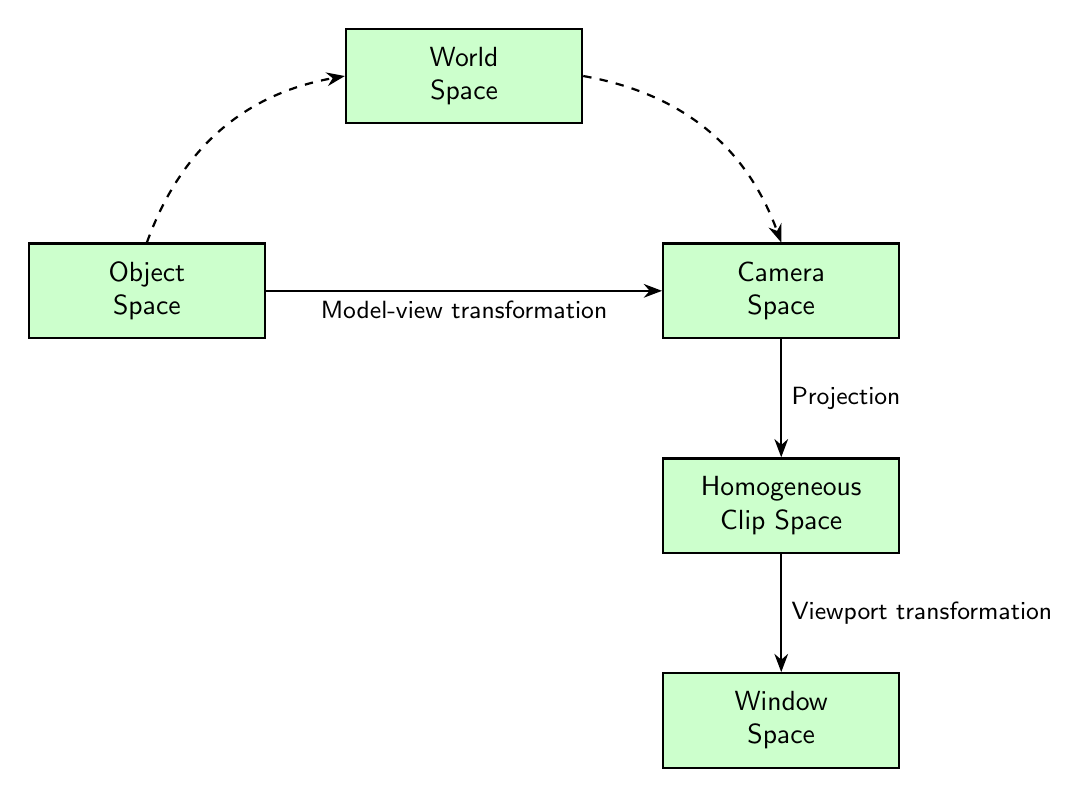
\begin{tikzpicture}[
    node distance=1.5cm and 2cm,
    box/.style={
        rectangle, 
        draw, 
        fill=green!20, 
        minimum width=3cm, 
        minimum height=1.2cm, 
        align=center,
        font=\sffamily,
        thick
    },
    arrow/.style={
        -Stealth, 
        thick,
        font=\sffamily\small
    },
    dashed_arrow/.style={
        -Stealth, 
        thick, 
        dashed,
        font=\sffamily\small
    }
]

% Nodes
\node[box] (object) {Object\\Space};
\node[box, above right=1.5cm and 1cm of object] (world) {World\\Space};
\node[box, below right=1.5cm and 1cm of world] (camera) {Camera\\Space};
\node[box, below=1.5cm of camera] (clip) {Homogeneous\\Clip Space};
\node[box, below=1.5cm of clip] (window) {Window\\Space};

% Solid Arrows
\draw[arrow] (object) -- (camera) node[midway, below] {Model-view transformation};
\draw[arrow] (camera) -- (clip) node[midway, right] {Projection};
\draw[arrow] (clip) -- (window) node[midway, right] {Viewport transformation};

% Dashed Curved Arrows
\draw[dashed_arrow] (object.north) to[bend left] (world.west);
\draw[dashed_arrow] (world.east) to[bend left] (camera.north);

\end{tikzpicture}
\end{document}
